\section{Result 5: with 32 bits per animal, runs stood still so long that they looked finished}
\label{sec:round32}

The first round could not test your idea, because no model was full. The only way left to press
the models harder was the 32-bit round. We had agreed to run it only if the first round
supported the idea, which it did not. I ran it all the same, because you told me during the
night to run everything.

\textbf{What changed.} Each animal now has its four facts for each of four seasons: 16 facts
in place of 4, and 32 bits in place of 8. Four words are added (\s{winter spring summer fall}),
and every sentence begins with a season: \s{in winter foxes eat meat .} An animal's facts in one
season have nothing to do with its facts in another. Every animal in every language of this
round carries the same 32 bits. A set is now four times as long, so that it still brings up
each fact of the largest language 15 times.

\textbf{How full the models would be.} I count, as in section \ref{sec:model}, only the numbers
a model really uses: its body and the rows of the words of its own language. By the rough guide
a model that learned all 256 animals would then be 85\% full at width 8, about one-third full
at width 16 and about one-tenth full at width 32. (That is as many bits as the 1,024 animals
of the first round, where width 8 came to 37\%. It is fuller now because it has only 256 animal
rows to keep them in.) With 1,024 animals the figures are 149\%, 66\% and 26\%.

\textbf{With 16 animals nothing changed.} Widths 8, 16 and 32 learned every fact, in both
repeats that I ran, within 16 to 64 sets.

\textbf{With 256 animals, the first runs looked like a failure.} I ran the agreed procedure
once for each width (the lines marked ``first run'' in table \ref{tab:large}). Widths 16 and 32
rose quickly to a score of 37 and stayed there, and the stopping test ended them as flat. Width
8 rose slowly, passed them, and was at 59 when its time ran out. (Its limit was first 15
minutes, in which it reached 48 after 174 sets; I replayed it with 40 minutes, because it was
the one run still climbing.) For width 16 the first two parts of our rule held: it had learned the 16
animals, and on 256 animals its run ended flat at a far lower score. The third part failed:
the model twice as wide did no better, with the same 37. By our agreement that means something
other than size was holding width 16 back. (For width 32 the rule cannot be asked, because I
ran no width 64.)

\begin{table}[t]
\centering\small
\begin{tabular}{@{}rrlcrrl@{}}
\toprule
Animals & Width & Run & ``Flat'' ending & Sets & Facts known & How it ended \\
\midrule
256 & 8 & repeat 1, first run & on & 445 & 59.2 & time ran out \\
256 & 8 & repeat 1, run again & off & 776 & 44.1 & time ran out \\
256 & 8 & repeat 2 & off & 391 & 34.8 & time ran out \\
\addlinespace[2pt]
256 & 16 & repeat 1, first run & on & 128 & 37.3 & ended as flat \\
256 & 16 & repeat 1, run again & off & 512 & 98.6 & fixed length reached \\
256 & 16 & repeat 2 & off & 91 & 99.9 & solved \\
\addlinespace[2pt]
256 & 32 & repeat 1, first run & on & 91 & 37.2 & ended as flat \\
256 & 32 & repeat 1, run again & off & 64 & 100.0 & solved \\
\addlinespace[2pt]
1{,}024 & 16 & repeat 1 & off & 328 & 93.6 & time ran out \\
\addlinespace[2pt]
1{,}024 & 32 & repeat 1 & off & 436 & 89.2 & time ran out \\
\bottomrule
\end{tabular}

\caption{The runs on the two large languages of the 32-bit round. A \emph{repeat} is a fresh
start: new starting numbers, new order of the text and new invented facts. ``Run again'' means
the same start and the same text once more: an exact replay for width 16, a different course
for widths 8 and 32 (see the text). With the ``flat'' ending on, the stopping test of section
\ref{sec:score} could end a run as flat. A fixed length is a number of sets set in advance.}
\label{tab:large}
\end{table}

\textbf{What a score of 37 is: these models took no notice of the season.} A score of 37 is 53
facts in 100 right (remember that 0 on our score already stands for 25 in 100). It is also
exactly what a model scores if it ignores the season word. Take one animal and one kind of
fact, say what foxes eat. The right answer differs from season to season. The two models that
stopped named the same food for all four seasons, and did so for 99\% of the animals and kinds
of fact. The food they named was
always the one that is right in more seasons than any other. They had learned what each animal
is \emph{usually} like, and nothing more.

\textbf{The stand-still was not the end.} Section \ref{sec:round1} had shown a model that
stood still for a long time and then moved again. So I ran width 16 on the 256 animals again
from the same start, this time for a fixed 512 sets and with the stopping test switched off.
A run can be replayed exactly: from the same start, on the same text, with the computer set up
the same way, a model takes exactly the same steps again. So this shows what the stopped run
would have done had I let it go on. From set 32 to set 362 its score
stayed at about 37. At set 512 it was 98.6, and it now gave different answers in
different seasons, as it should. The ``flat'' ending had been wrong: the test had ended this
model at set 128, and its stand-still lasted until some point after set 362.

That changed my plan for the rest of the night. More short runs under the same stopping test
would only have given more wrong endings. I dropped them and ran the models for as long as the
night allowed with the ``flat'' ending switched off: the first repeat again and, for widths 8
and 16, a second repeat (table \ref{tab:large}, figure \ref{fig:large}).

\begin{figure}[t]
\centering
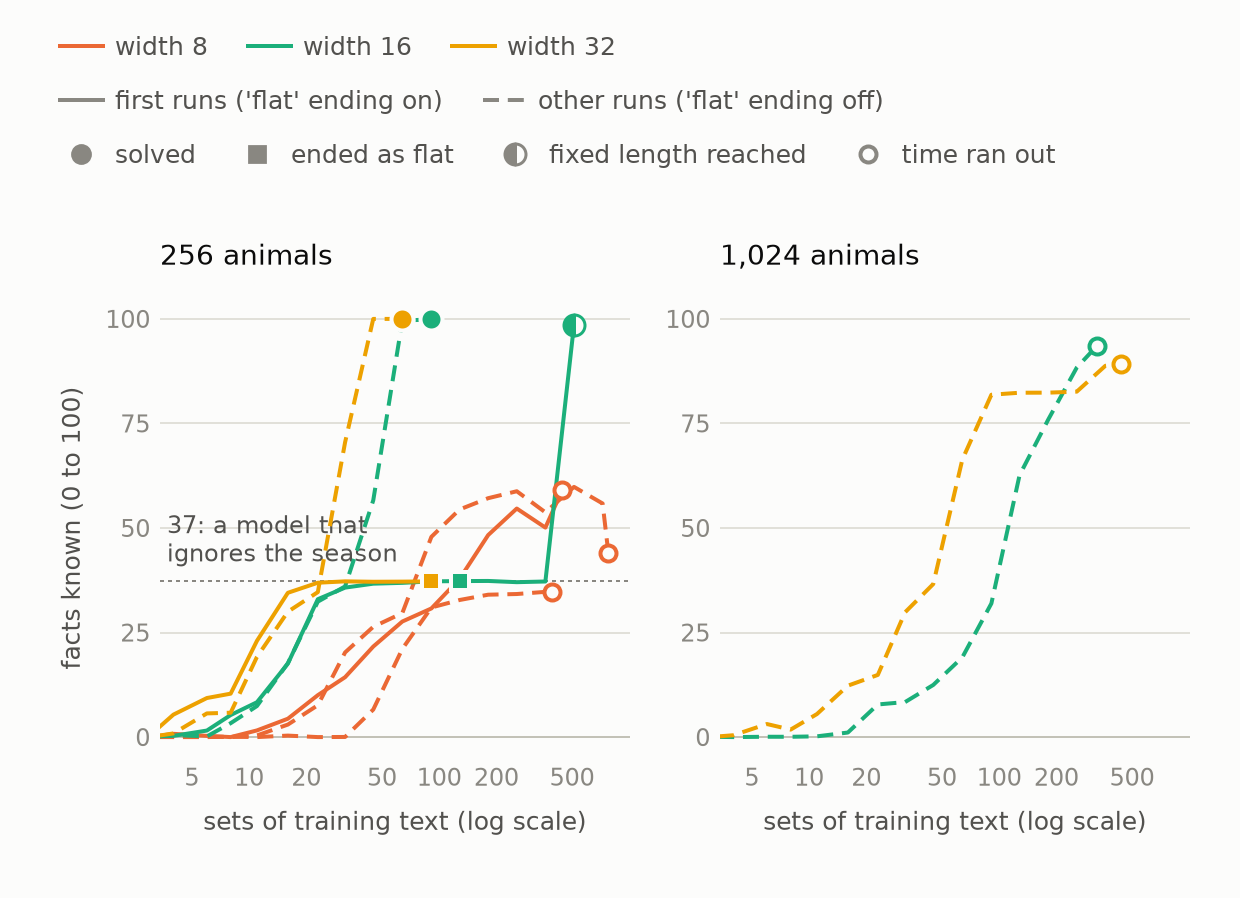
\includegraphics[width=0.68\textwidth]{figures/large_equal_x4.png}
\caption{The runs of table \ref{tab:large}, as training went on. Solid lines are the first
runs. The first run of width 16 is drawn as its exact retrace, which went on to 512 sets; the
square on it marks set 128, where the stopping test had ended it as flat. Dashed lines are the
other runs. The dotted line at 37 is the score of a model that ignores the season.}
\label{fig:large}
\end{figure}

\textbf{Whether a run stood still was a matter of chance.} Widths 16 and 32 made four different
attempts at the 256 animals. (The 512-set run retraced one of them exactly, so I do not count
it.) Two stood still at 37: the two first runs. Two went straight through and were solved
after 91 and 64 sets. The two runs of width 32 make the point most plainly. They started from
the same numbers and read the same text; for the second the computer was only set up
differently (it used a different number of its processors), which changes the last digits of
the arithmetic and nothing else. The first
was still standing at 37 when the test ended it at set 91. The second passed 37 without a
pause and knew every fact by set 45.

\textbf{Width 8 is the one place where your prediction may be showing.} By the rough guide it
would be 85\% full if it learned all 256 animals. That is under the limit, but the guide is
rough and comes from far larger models. Width 8 did not learn them in any of its three runs
(two repeats, the first of them run twice). In the first repeat it was at 59 after 445 sets;
run again, it kept shifting between 54 and 60 from set 128 to set 724 and was at 44 at its
last grading, set 776. In the second repeat it never came to use the season and stood between
33 and 35 from set 128 to its end. Width 16 reached 98.6 and 99.9 in the same two repeats, and
width 32 reached 100 in the one repeat it had. So here a model does do worse on more words, and wider models do better.

What width 8 knew is the most telling thing about it. The next figures are plain counts of
right answers in 100, not scores: guessing gives 25, and a model that ignores the season 53.
Both sets of figures come from the first repeat: its first run, and the same start run again
with the computer set up differently, which took a course of its own. When the first run
stopped, width 8 had 89 of the foods and 78 of the homes right, but only 57 of the colors and
54 of the waking times. When the second stopped, it had 93 of the homes and 81 of the waking
times, but only 34 of the foods and 25 of the colors. So the two runs held different pairs of
the four kinds of fact, and the second lost 12 points of score between its last two gradings.
It looks as if width 8 can hold about two of the four kinds at a time. That is what a model
that is too small would look like.

I still do not count it as support under our rule. The rule needs a run that ends flat by our
test, and none of the three did when I put the test to their saved scores afterwards. The two
runs of the first repeat never settled: their scores kept shifting by several points from one
grading to the next. The
second repeat did stand still, but its time ran out before it had stood still long enough for
the test to call it flat. And it was standing where we have seen models stand before: it took
no notice of the season, and other models went on from there in the end. But it is the best
lead of the night.

\textbf{On 1,024 animals,} which I had left out for lack of time, the cores that came free
allowed one long run each of widths 32 and 16. Both were still rising when their time ran out,
so they say nothing yet about limits. Width 16 was at 94 after 328 sets. Width 32 rose to 82
by set 91, stood there until set 256 while width 16 overtook it, and then moved again, to 89
at set 436. (At the end the homes were the one kind of fact it had not yet learned.)

\textbf{What this round says.} The verdict by the rule stays undecided: no run of width 8
ended flat, and where the first two parts of the rule did hold, for the first runs of widths
16 and 32, it was by a wrong ending. One caution about the lead at width 8: this round changed two things
at once. Each animal had four times as much to be remembered, and no fact could be answered
from the animal word alone any more, because the model had to put the animal and the season
together. These runs cannot tell me which of the two made the larger languages so much harder.
